\documentclass[aspectratio=169,11pt]{beamer}
\usepackage[T1]{fontenc}
\usepackage{lmodern}
\usepackage{booktabs}
\usepackage{array}
\usepackage{amsmath,amssymb}
\graphicspath{{../results/}}
% generated by analysis/run_all.py; do not edit
\newcommand{\NProposals}{351}
\newcommand{\NExecuted}{281}
\newcommand{\NDefeated}{33}
\newcommand{\NCanceled}{37}
\newcommand{\NDecided}{314}
\newcommand{\NVotes}{14,396}
\newcommand{\NPlayers}{4,912}
\newcommand{\NLive}{76}
\newcommand{\TopOneShare}{13.1\%}
\newcommand{\TopOneBz}{14.9\%}
\newcommand{\TopOneSS}{14.3\%}
\newcommand{\TopFiveShare}{38.2\%}
\newcommand{\TopFiveBz}{39.6\%}
\newcommand{\TopFiveSS}{40.6\%}
\newcommand{\NakShare}{10}
\newcommand{\NakSS}{9}
\newcommand{\MaxGapBz}{4.8}
\newcommand{\MaxGapSS}{2.2}
\newcommand{\TVBzSS}{0.015}
\newcommand{\TVBzSSmax}{0.026}
\newcommand{\TVShareBz}{0.022}
\newcommand{\TVShareSS}{0.020}
\newcommand{\SpearmanMin}{1.000}
\newcommand{\FlipOne}{118}
\newcommand{\FlipMedian}{2}
\newcommand{\FlipMax}{5}
\newcommand{\TopkOne}{26.4\%}
\newcommand{\TopkThree}{73.2\%}
\newcommand{\TopkFive}{97.5\%}
\newcommand{\TopkTen}{100.0\%}
\newcommand{\Turnout}{25.5\%}
\newcommand{\ResDiff}{0.00016}
\newcommand{\TransMoved}{5.3\%}
\newcommand{\DummyMax}{0.1\%}
\newcommand{\TopOneExceeds}{100.0\%}
\newcommand{\DelegMismatch}{0}
\newcommand{\VoteMismatch}{0}
\newcommand{\DefeatedFlipOne}{28}


% ---- minimal clean style
\usetheme{default}
\setbeamertemplate{navigation symbols}{}
\definecolor{ink}{HTML}{0B0B0B}
\definecolor{ink2}{HTML}{52514E}
\definecolor{accent}{HTML}{2A78D6}
\definecolor{accent2}{HTML}{EB6834}
\definecolor{surface}{HTML}{FCFCFB}
\setbeamercolor{background canvas}{bg=surface}
\setbeamercolor{normal text}{fg=ink}
\setbeamercolor{frametitle}{fg=ink}
\setbeamercolor{title}{fg=ink}
\setbeamercolor{structure}{fg=accent}
\setbeamercolor{alerted text}{fg=accent2}
\setbeamerfont{frametitle}{series=\bfseries,size=\Large}
\setbeamertemplate{itemize items}{\raisebox{0.15em}{\scriptsize$\blacksquare$}}
\setbeamertemplate{footline}{\hfill\textcolor{ink2}{\scriptsize\insertframenumber\,/\,\inserttotalframenumber}\hspace{1em}\vspace{0.6em}}
\newcommand{\muted}[1]{\textcolor{ink2}{#1}}

\title{Who actually decides?\\[0.2em]\large Measuring voting-power concentration in Compound governance}
\author{Ashik Stenny \and Aarav Oswal\\[0.3em]\small Group 14 \textperiodcentered{} CS731 Blockchain Technology and Applications \textperiodcentered{} IIT Kanpur}
\date{28 October 2026}

\begin{document}

\begin{frame}
  \titlepage
\end{frame}

% =================================================================== 1. Problem
\section{Problem}
\begin{frame}{Token voting looks decentralised}
  \begin{itemize}
    \item DAOs govern protocols holding billions of dollars by token-weighted on-chain votes.
    \item Compound: anyone holding COMP can vote, directly or by delegating.
    \item The usual decentralisation metrics are \textbf{token share} and the Gini coefficient.
  \end{itemize}
  \vspace{1em}
  \textbf{But token share is not decision power.}
  \begin{itemize}
    \item A 49\% holder facing one 51\% holder has \emph{no} power; facing 51 holders of 1\% each, it has almost all.
    \item Power depends on \emph{who else} holds weight, the \emph{quota}, and \emph{delegation}.
  \end{itemize}
  \vspace{1em}
  \muted{Question: how far apart are nominal share and effective power in a real DAO, and how often did a handful of addresses decide outcomes?}
\end{frame}

\begin{frame}{What we did}
  \begin{enumerate}
    \item Rebuilt \textbf{every} Compound GovernorBravo proposal (\NProposals) and vote (\NVotes) from raw Ethereum logs.
    \item Reconstructed each delegate's voting weight at each proposal's snapshot by \textbf{replaying all 2.33M COMP transfers and 16k delegation events}.
    \item Implemented delegation resolution, \textbf{Banzhaf} and \textbf{Shapley--Shubik} indices by dynamic programming ourselves (no index library).
    \item Compared token share against both indices, and the indices against what actually happened in each vote.
  \end{enumerate}
  \vspace{0.8em}
  \muted{Everything is reproducible from one config file and five commands; every number on these slides is generated by a script.}
\end{frame}

% =================================================================== 2. Background
\section{Background}
\begin{frame}{Weighted voting games}
  \begin{itemize}
    \item Players $N=\{1,\dots,n\}$ with weights $w_i \ge 0$ and a quota $q$.
    \item A coalition $S$ \textbf{wins} iff $w(S)=\sum_{i\in S} w_i \ge q$. Written $[q;\,w_1,\dots,w_n]$.
    \item Player $i$ \textbf{swings} for $S \subseteq N\setminus\{i\}$ if $S$ loses but $S\cup\{i\}$ wins:
      \[ q - w_i \;\le\; w(S) \;<\; q. \]
  \end{itemize}
  \vspace{0.5em}
  \textbf{Example} $[51;\,50,30,20]$: winning coalitions $\{1,2\},\{1,3\},\{1,2,3\}$.\\
  Player 1 holds 50\% of the weight but is in every winning coalition.
\end{frame}

\begin{frame}{Two power indices}
  \small
  \textbf{Banzhaf}: how often is $i$ a swing, over all coalitions of the others?
  \[ \psi_i = \frac{\#\{S \subseteq N\setminus\{i\} : q-w_i \le w(S) < q\}}{2^{\,n-1}}, \qquad \beta_i = \frac{\psi_i}{\sum_j \psi_j}. \]
  \textbf{Shapley--Shubik}: in a random ordering of players, how often is $i$ the one whose arrival first reaches $q$?
  \[ \varphi_i = \sum_{\substack{S \subseteq N\setminus\{i\}\\ q-w_i \le w(S) < q}} \frac{|S|!\,(n-1-|S|)!}{n!}. \]
  \begin{center}
  \begin{tabular}{lccc}
    \toprule
    $[51;\,50,30,20]$ & player 1 & player 2 & player 3\\ \midrule
    token share & 0.50 & 0.30 & 0.20\\
    Banzhaf $\beta$ & 0.60 & 0.20 & 0.20\\
    Shapley--Shubik $\varphi$ & 0.667 & 0.167 & 0.167\\ \bottomrule
  \end{tabular}
  \end{center}
  \vspace{-0.4em}
  \muted{\footnotesize (The project brief listed $\beta=(0.50,0.25,0.25)$; enumeration gives 3, 1, 1 swings, so $(0.6,0.2,0.2)$.)}
\end{frame}

\begin{frame}{Delegation in COMP}
  \begin{itemize}
    \item A holder's tokens vote only if it \textbf{delegates}, to itself or to another address.
    \item Delegation is \textbf{one-hop}: if $A\to B$ and $B\to C$, then $A$'s tokens count for $B$, and $B$'s own tokens for $C$.
    \item Undelegating ($\to$ \texttt{0x0}) removes the votes; undelegated tokens count for nobody.
    \item Voting weight at a proposal = $\sum$ balances delegated to you, at its \texttt{startBlock}.
  \end{itemize}
  \vspace{0.6em}
  \textbf{Our resolver} implements this rule, plus a \emph{transitive} variant for sensitivity:
  \begin{itemize}
    \item follow $A\to B\to C\to\cdots$ to a self-delegated or non-delegating address;
    \item \textbf{cycle rule:} addresses on a cycle are treated as self-delegated; a chain entering a cycle stops at the first cycle address.
  \end{itemize}
\end{frame}

% =================================================================== 3. What is done
\section{What is done}
\begin{frame}{Pipeline}
  \small
  \begin{center}
  \begin{tabular}{p{0.26\textwidth}p{0.66\textwidth}}
    \toprule
    \textbf{Stage} & \textbf{What it does}\\ \midrule
    \texttt{data.fetch} & \texttt{eth\_getLogs} for 8 event types over blocks 9.6M--22.0M, adaptive range splitting, cached to \texttt{data/raw/} (175 MB)\\
    \texttt{data.process} & ABI-decode; replay transfers + delegations in one pass over all snapshots; write CSVs\\
    \texttt{power/} & delegation resolver, Banzhaf DP, Shapley--Shubik DP, flip sets, gap metrics\\
    \texttt{analysis.run\_all} & all tables, figures, and the numbers on these slides\\ \bottomrule
  \end{tabular}
  \end{center}
  \vspace{0.6em}
  \begin{itemize}
    \item Scope: Compound GovernorBravo, proposals 43--393 (\NExecuted{} executed, \NDefeated{} defeated, \NCanceled{} canceled).
    \item Players: every address with positive voting weight at the snapshot (median \NPlayers{} per proposal).
    \item Quota: pass iff for $>$ against and for $\ge$ 400k COMP $\Rightarrow$ $q=\max(\lfloor W/2\rfloor+1,\;Q)$.
  \end{itemize}
\end{frame}

\begin{frame}{The data is exact}
  We never trust a third-party API for weights; instead we check our reconstruction against the chain itself.
  \vspace{0.8em}
  \begin{center}
  \begin{tabular}{p{0.78\textwidth}r}
    \toprule
    Check & Mismatches\\ \midrule
    Our delegate weights vs on-chain checkpoints (all delegates, \NProposals{} snapshots) & \textbf{\DelegMismatch}\\
    Our weight vs the weight of each of the \NVotes{} \texttt{VoteCast} events & \textbf{\VoteMismatch}\\
    Our for/against/abstain tallies vs \texttt{proposals(id)} & \textbf{0}\\
    Our outcome label vs \texttt{state(id)} & \textbf{0}\\ \bottomrule
  \end{tabular}
  \end{center}
  \vspace{0.8em}
  \muted{This validates the delegation resolver and the snapshot rule (events in block $\le$ \texttt{startBlock}) end to end.}
\end{frame}

\begin{frame}{Computing the indices: dynamic programming}
  \small
  \textbf{Banzhaf.} $p[x]=\Pr(w(S)=x)$ for $S$ a random subset; add a player of weight $v$:
  \[ p'[x] = \tfrac12\big(p[x] + p[x-v]\big), \qquad x < q. \]
  \textbf{Shapley--Shubik.} $P[k,x]=\Pr(w(S)=x)$ for $S$ a random $k$-subset of the $m$ players so far:
  \[ P'[k,x] = \frac{(m+1-k)\,P[k,x] + k\,P[k-1,x-v]}{m+1}, \]
  \[ \varphi_i = \frac1n \sum_{k=0}^{n-1} \Pr\nolimits_k\big(q-w_i \le w(S) < q\big). \]
  \begin{itemize}
    \item Convex combinations: no overflow, even for thousands of players (raw counts reach $\binom{n}{n/2}$).
    \item Leave-one-out by \textbf{divide and conquer} over distinct weights: only additions, no unstable ``removal''.
    \item Weights rounded to $W/20000$; dummies carry $\le$ \DummyMax{} of weight. Changing the resolution moves any index by $\le$ \ResDiff.
  \end{itemize}
\end{frame}

\begin{frame}{Tests (280, all passing)}
  \begin{columns}[T]
  \begin{column}{0.5\textwidth}
  \textbf{Indices}
  \begin{itemize}
    \item known example $[51;50,30,20]$ to $10^{-9}$
    \item dummy players get 0
    \item equal weights $\Rightarrow$ equal indices
    \item Shapley--Shubik sums to 1
    \item DP $=$ brute force on 40 random games with $n\le 12$
    \item DP $=$ permutation definition ($n\le 7$)
  \end{itemize}
  \end{column}
  \begin{column}{0.5\textwidth}
  \textbf{Delegation \& outcomes}
  \begin{itemize}
    \item chains, cycles, self-delegation, undelegation, re-delegation
    \item same-block ordering by log index
    \item snapshot unaffected by later events
    \item one-pass replay $=$ direct recomputation
    \item minimal flip set $=$ brute force on 200 random votes
  \end{itemize}
  \end{column}
  \end{columns}
  \vspace{1em}
  \muted{\texttt{pytest} runs in about 2 seconds.}
\end{frame}

% =================================================================== 4. Results
\section{Results}
\begin{frame}{A few delegates hold most of the weight}
  \begin{columns}[c]
  \begin{column}{0.35\textwidth}
    Median over \NProposals{} proposals:\\[0.6em]
    \begin{tabular}{lr}
      \toprule
      & largest delegate\\ \midrule
      token share & \TopOneShare\\
      Banzhaf & \TopOneBz\\
      Shapley--Shubik & \TopOneSS\\ \bottomrule
    \end{tabular}\\[0.8em]
    Top 5: \TopFiveShare{} of weight, \TopFiveBz{} / \TopFiveSS{} of power.\\[0.5em]
    Of \NPlayers{} players, only $\sim$\NLive{} are not dummies.
  \end{column}
  \begin{column}{0.6\textwidth}
    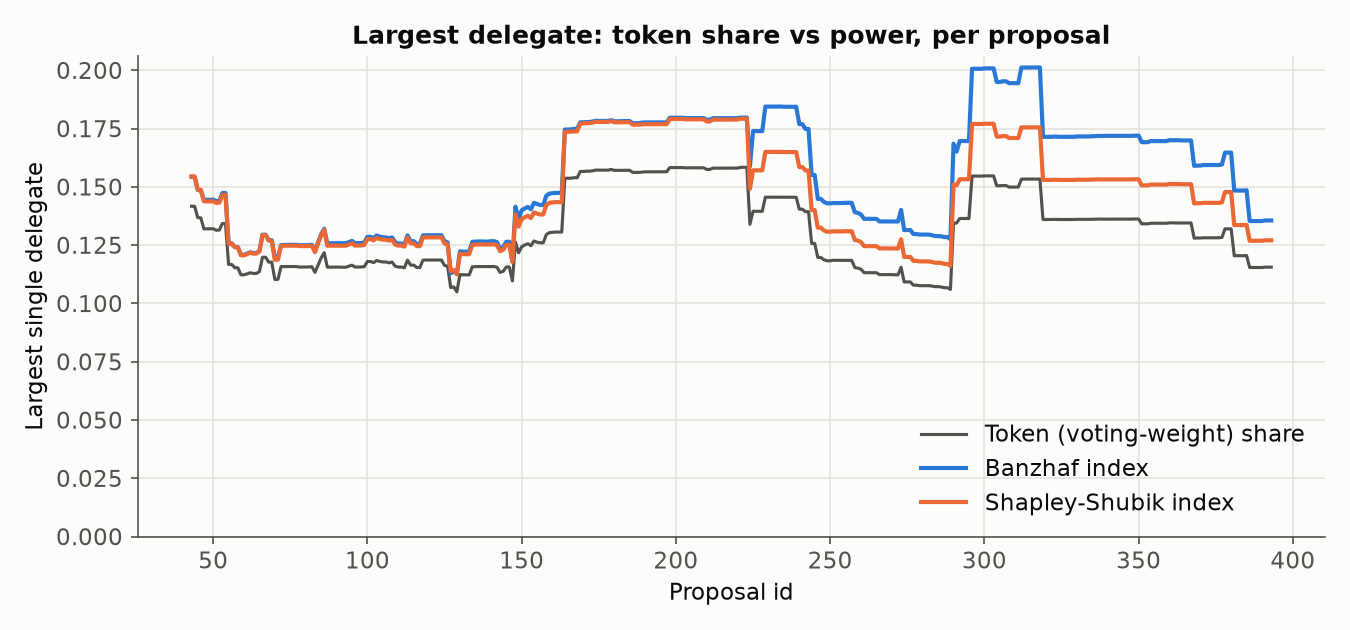
\includegraphics[width=\textwidth]{fig_top1_power.png}
  \end{column}
  \end{columns}
\end{frame}

\begin{frame}{Nominal vs effective: the largest are amplified}
  \begin{columns}[c]
  \begin{column}{0.34\textwidth}
    \begin{itemize}
      \item The 1--2 largest delegates get $\approx 1.1\times$ power per unit of tokens.
      \item Nearly everyone else is compressed to $\approx 0.96\times$.
      \item Largest single gap: $+\MaxGapBz$ points (Banzhaf), $+\MaxGapSS$ points (Shapley--Shubik), both for the top delegate.
    \end{itemize}
  \end{column}
  \begin{column}{0.64\textwidth}
    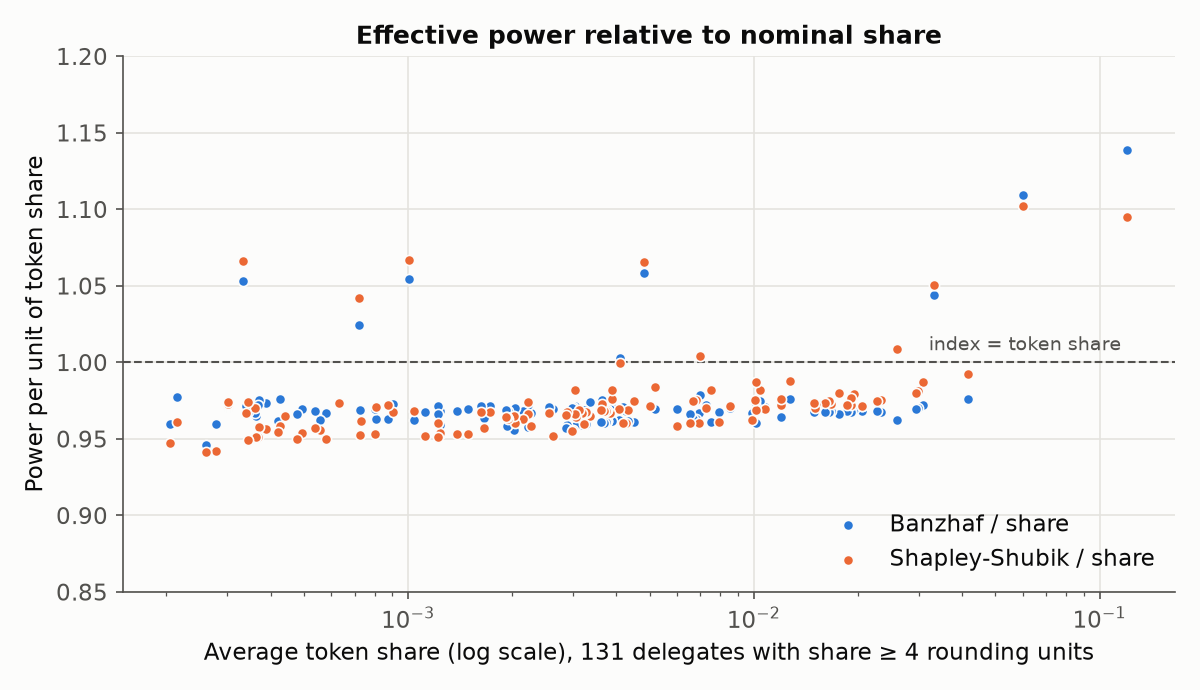
\includegraphics[width=\textwidth]{fig_gap_scatter.png}
  \end{column}
  \end{columns}
\end{frame}

\begin{frame}{Ten largest delegates}
  \centering
  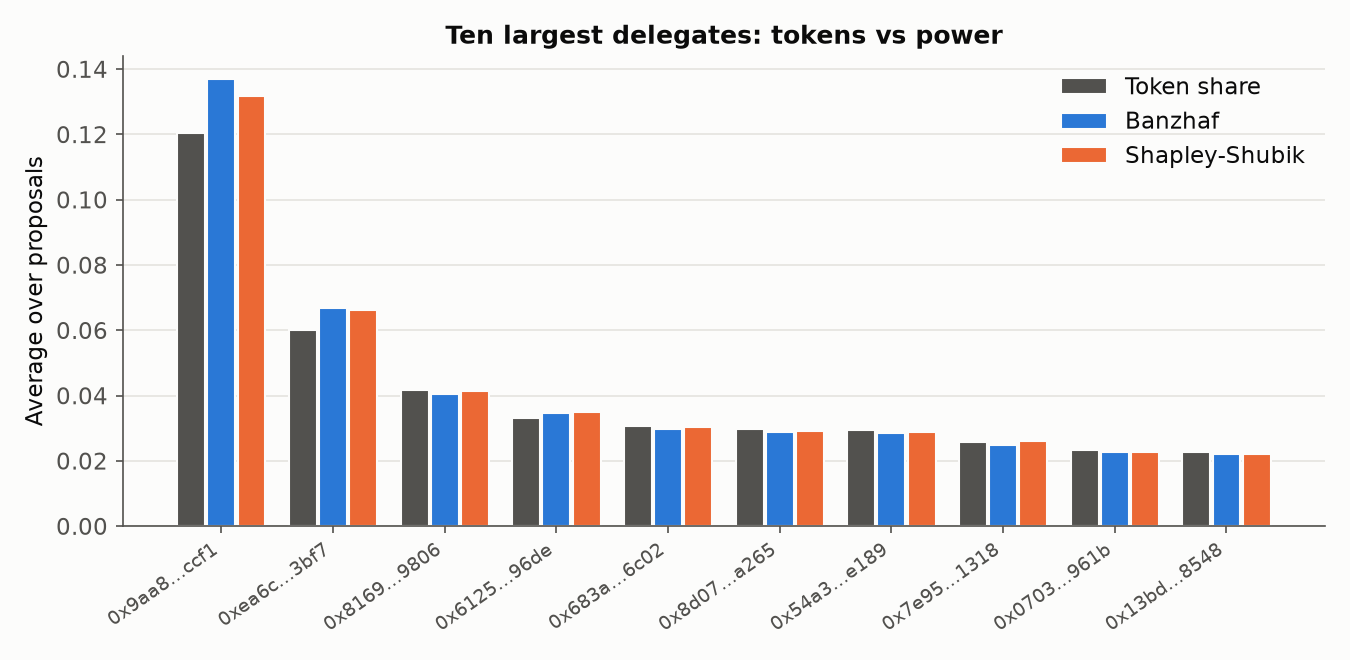
\includegraphics[width=0.86\textwidth]{fig_top10_delegates.png}\\
  \muted{\small Averaged over all proposals. Addresses are shown, not identities: one entity may control several.}
\end{frame}

\begin{frame}{Banzhaf vs Shapley--Shubik: same order, different sizes}
  \begin{columns}[c]
  \begin{column}{0.36\textwidth}
    \begin{itemize}
      \item Spearman rank correlation is \SpearmanMin{} in \emph{every} proposal.
      \item That is a theorem: in a weighted game, a heavier player is always at least as powerful under both indices.
      \item The real difference is in magnitude: total-variation distance median \TVBzSS{} (max \TVBzSSmax).
      \item Banzhaf favours the top delegate more after proposal $\sim$225.
    \end{itemize}
  \end{column}
  \begin{column}{0.62\textwidth}
    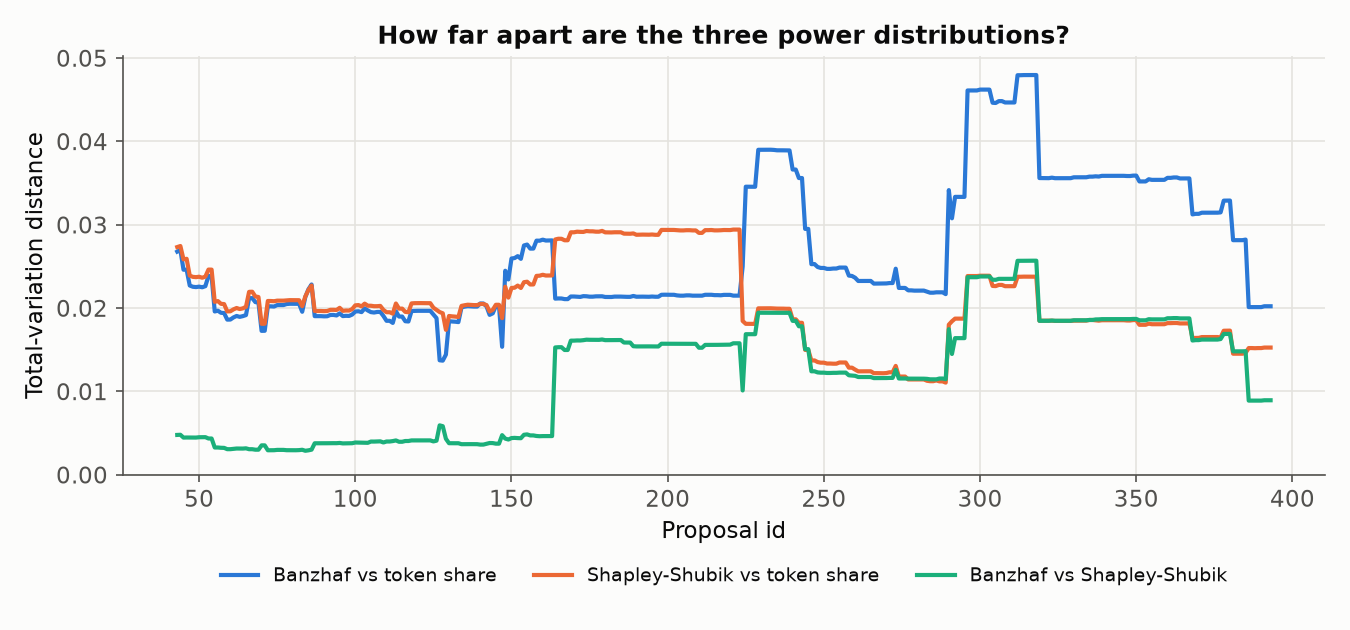
\includegraphics[width=\textwidth]{fig_distribution_distance.png}
  \end{column}
  \end{columns}
\end{frame}

\begin{frame}{From power to outcomes: how many addresses decided?}
  \begin{columns}[c]
  \begin{column}{0.38\textwidth}
    \textbf{Flip set}: players who, changing only their own votes, reverse the result (with quorum).\\[0.6em]
    Of \NDecided{} decided proposals:
    \begin{itemize}
      \item \textbf{\FlipOne} could be reversed by \textbf{one} address
      \item median minimal set: \FlipMedian{}; never more than \FlipMax
      \item \DefeatedFlipOne{} of \NDefeated{} defeated proposals: one large non-voter could have passed them
    \end{itemize}
  \end{column}
  \begin{column}{0.6\textwidth}
    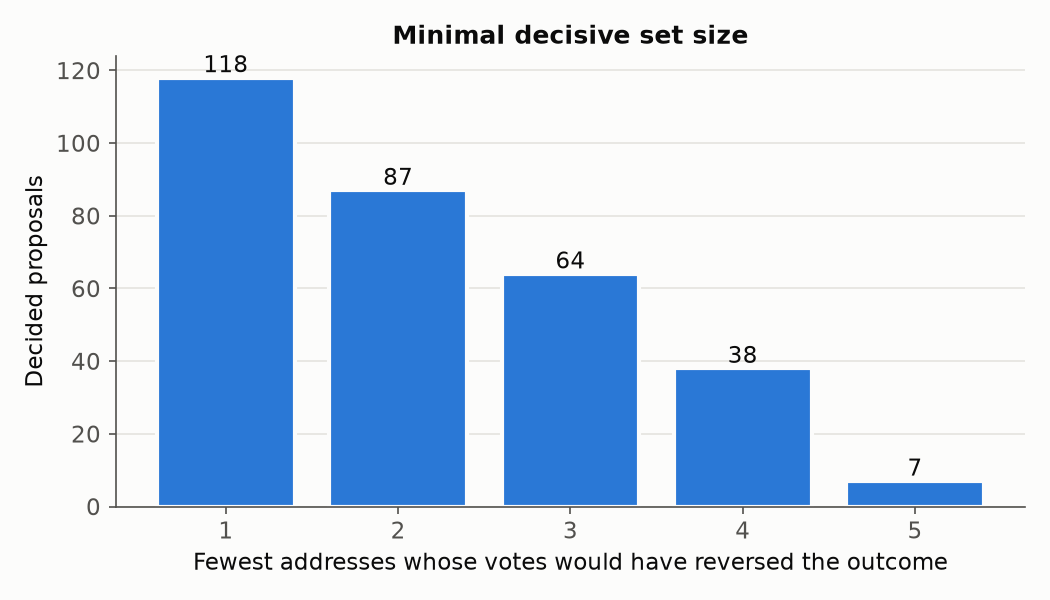
\includegraphics[width=\textwidth]{fig_min_flip_size.png}
  \end{column}
  \end{columns}
\end{frame}

\begin{frame}{Could the top-$k$ have reversed it alone?}
  \begin{columns}[c]
  \begin{column}{0.34\textwidth}
    \begin{tabular}{rr}
      \toprule
      $k$ & share of outcomes\\ \midrule
      1 & \TopkOne\\
      3 & \TopkThree\\
      5 & \TopkFive\\
      10 & \TopkTen\\ \bottomrule
    \end{tabular}\\[1em]
    Median turnout: \Turnout{} of delegated weight. Low turnout is what makes a few large delegates decisive.
  \end{column}
  \begin{column}{0.64\textwidth}
    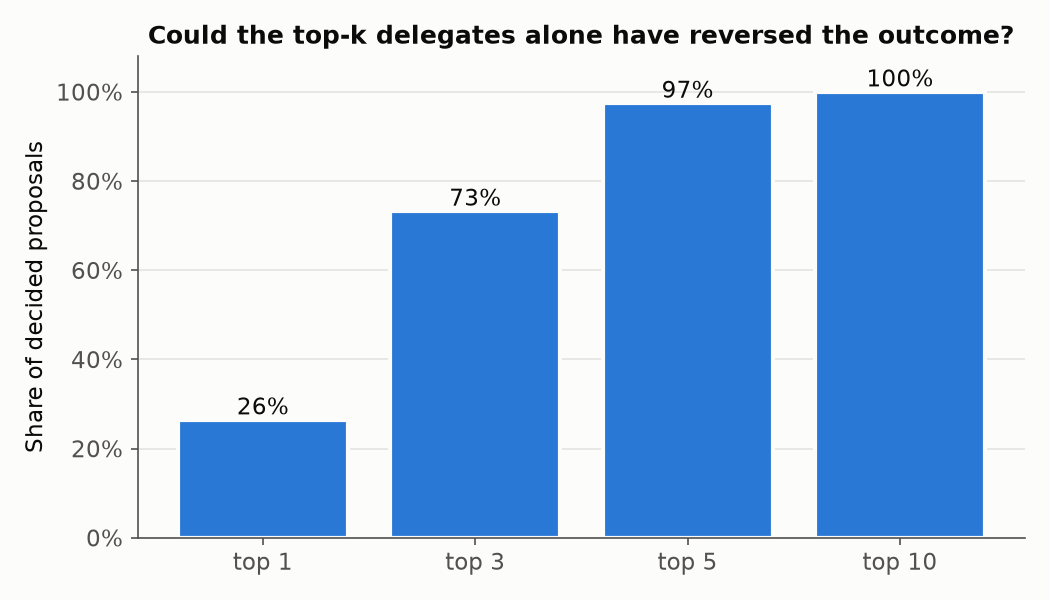
\includegraphics[width=\textwidth]{fig_topk_pivotal.png}
  \end{column}
  \end{columns}
\end{frame}


\begin{frame}{Beyond the base game: power among those who actually vote}
  \begin{columns}[c]
  \begin{column}{0.36\textwidth}
    \small
    Players = the \textbf{for/against voters} only; same quota rule on votes cast.
    \begin{itemize}
      \item Quorum (400k COMP) now binds in \PartQuorumBinds{} of \PartGames{} decided proposals.
      \item In \PartNoWin, the voters could not reach quorum at all.
      \item Median: \PartVoters{} voters; the largest holds \PartTopOneShare{} of cast votes but \PartTopOneSS{} Shapley--Shubik power.
      \item Nakamoto (Shapley--Shubik) drops from \NakSS{} to \PartNakSS.
    \end{itemize}
  \end{column}
  \begin{column}{0.62\textwidth}
    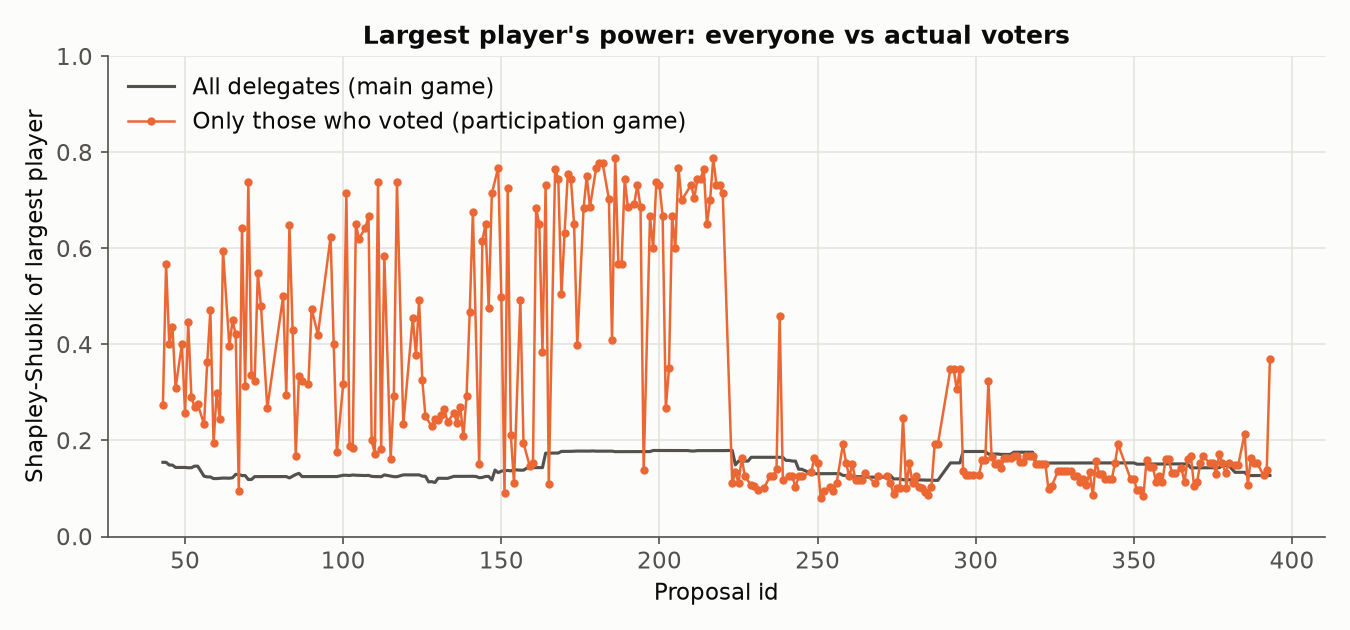
\includegraphics[width=\textwidth]{fig_participation_power.png}
  \end{column}
  \end{columns}
\end{frame}

\begin{frame}{Agreement with prior work}
  We recomputed the published Compound metrics on our own data.
  \vspace{0.8em}
  \begin{center}
  \small
  \begin{tabular}{>{\raggedright\arraybackslash}p{0.27\textwidth}>{\raggedright\arraybackslash}p{0.33\textwidth}cc}
    \toprule
    Source & Metric & Published & Ours\\ \midrule
    Fritsch, M\"uller \& Wattenhofer (2022) & Nakamoto coefficient of delegates, block 14.3M & 8 & \textbf{\NakFritsch}\\[0.3em]
    Fritsch, M\"uller \& Wattenhofer (2022) & Gini coefficient of delegates, block 14.3M & 0.987 & \textbf{\GiniFritsch}\\[0.3em]
    Messias et al.\ (2023) & mean voters needed for $\ge$50\% of votes cast & 3.18 & \textbf{\VotersHalf}\\ \bottomrule
  \end{tabular}
  \end{center}
  \vspace{0.6em}
  \begin{itemize}
    \item Ours: snapshot block \FritschBlock{}; \VotersHalfN{} decided Bravo proposals. Messias et al.\ also include Governor Alpha and data to Aug 2024.
    \item \textbf{What we add:} neither paper computes Banzhaf or Shapley--Shubik indices. Fritsch et al.\ use ``could one delegate flip this vote''; we compute both indices exactly over the delegation-resolved game, for every proposal.
  \end{itemize}
\end{frame}

\begin{frame}{Their power measure vs our indices}
  \small
  \textbf{Potential power} (Fritsch et al., Def.\ 4.1): could this voter, by switching its vote, have flipped the result? \textbf{Exercised power} (Def.\ 4.2): did removing its vote flip it?
  \vspace{0.4em}
  \begin{columns}[T]
  \begin{column}{0.48\textwidth}
    \textbf{On our data} (Compound rule, with quorum)
    \begin{itemize}
      \item Only \PotVoters{} of \PotVotersTotal{} voters \emph{ever} had potential power, in \PotProposals{} of \NDecided{} proposals.
      \item One delegate could have flipped \PotTop{} of the \PotTopVoted{} proposals it voted on.
      \item Sanity check: every such proposal also has a one-address flip set in our analysis (asserted in code).
    \end{itemize}
  \end{column}
  \begin{column}{0.5\textwidth}
    \textbf{Why we need full indices}
    \begin{itemize}
      \item Potential power checks a swing at \emph{one} coalition, the one that happened. Banzhaf averages swings over \emph{all} $2^{n-1}$ coalitions; Shapley--Shubik over all orderings.
      \item It is 0 for most voters in most votes, so it cannot rank them; our indices can.
      \item Yet they agree: potential-power rate vs our Shapley--Shubik, Spearman \PotSpearman{} over \PotActive{} voters with $\ge$5 votes.
    \end{itemize}
  \end{column}
  \end{columns}
\end{frame}

\begin{frame}{Takeaways}
  \begin{enumerate}
    \item \textbf{Concentration is real, and slightly worse than token share suggests.} The top delegate's power exceeds its share under both indices in \TopOneExceeds{} of proposals; the median Nakamoto coefficient falls from \NakShare{} (weight) to \NakSS{} (Shapley--Shubik).
    \item \textbf{The two indices agree on who matters} (by theorem) and differ by only $\sim$\TVBzSS{} in total variation, but Banzhaf amplifies the top delegate more.
    \item \textbf{Among actual voters it is starker:} quorum binds in \PartQuorumBinds{} of \PartGames{} proposals and \PartNakSS{} voters hold most of the power.
    \item \textbf{Realised outcomes are fragile.} The top 5 delegates could have reversed \TopkFive{} of all decided proposals; a single address, \FlipOne{} of \NDecided.
  \end{enumerate}
\end{frame}

% =================================================================== 5. Limitations
\section{Limitations}
\begin{frame}{Limitations}
  \begin{itemize}
    \item \textbf{Snapshot choice:} weights at \texttt{startBlock}, exactly as the protocol counts; delegation can change during voting but cannot affect votes.
    \item \textbf{Delegation rule:} one-hop, as in COMP. A transitive reading moves at most \TransMoved{} of weight in any proposal.
    \item \textbf{Addresses $\ne$ people:} one entity may control many addresses, which would make concentration \emph{higher}. Fritsch et al.\ cluster addresses by transfers but call it ``not bullet-proof''; we do not cluster.
    \item \textbf{Model assumptions:} the index game assumes all players vote and are not strategic (no coordination). Real turnout is \Turnout; the participation game (slide on actual voters) relaxes the all-vote assumption.
    \item \textbf{Rounding:} integer weights at $W/20000$; effect $\le$ \ResDiff{} on any index.
    \item \textbf{Scope:} one DAO and one governor contract (GovernorBravo, 2021--2025).
  \end{itemize}
\end{frame}

% =================================================================== 6. Future
\section{Future directions}
\begin{frame}{Future directions}
  \begin{itemize}
    \item \textbf{Turnout models:} between our two games, weight players by their historical participation.
    \item \textbf{Entity clustering:} merge addresses controlled by the same organisation.
    \item \textbf{Second DAO:} Uniswap uses the same token/governor design, so the pipeline transfers with a config change.
    \item \textbf{Off-chain voting} (Snapshot) and liquid-delegation designs where chains really are transitive.
    \item \textbf{Mechanism design:} how quorum or vote caps would change the indices.
  \end{itemize}
  \vspace{1em}
  \muted{\small References: Fritsch, M\"uller \& Wattenhofer, \emph{Analyzing Voting Power in Decentralized Governance: Who controls DAOs?}, arXiv:2204.01176.\\
  Messias et al., \emph{Understanding Blockchain Governance: Analyzing Decentralized Voting to Amend DeFi Smart Contracts}, arXiv:2305.17655.}
\end{frame}

\begin{frame}
  \centering
  \vspace{2em}
  {\Huge\bfseries Thank you}\\[1.5em]
  \muted{Questions?}\\[2em]
  \small Code, data pipeline and all results: \texttt{README.md} section 10 reproduces every number.
\end{frame}

\end{document}
